\section{Benchmark}

\begin{frame}
\frametitle{Dataset and models Different models}
Datasets:
\begin{itemize}
    \item ImageNet
    \item ImageNet Real (better labeling)
    \item JFT-300M with 18k classes and 303M high-resolution images
    \item CIFAR-10 6k 32x32 colour images in 10 classes, with 6000 images per class
    \item CIFAR-100 100 classes containing 600 images each
    \item Oxford-IIIT Pet 37 category 200 images for each class
\end{itemize}
\vspace{0.4cm}

Models:
\begin{center}
    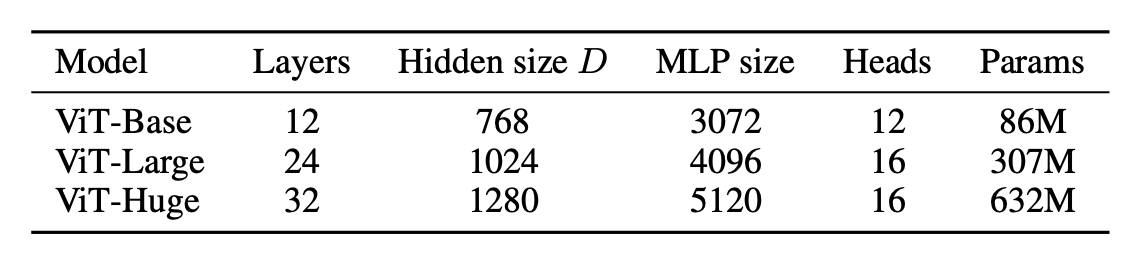
\includegraphics[width=0.8\textwidth]{img/3-section/Varianti VIT.png} 
\end{center}

\end{frame}

\begin{frame}
\frametitle{Results}
Comparison with state of the art on popular image classification benchmarks:
\begin{center}
    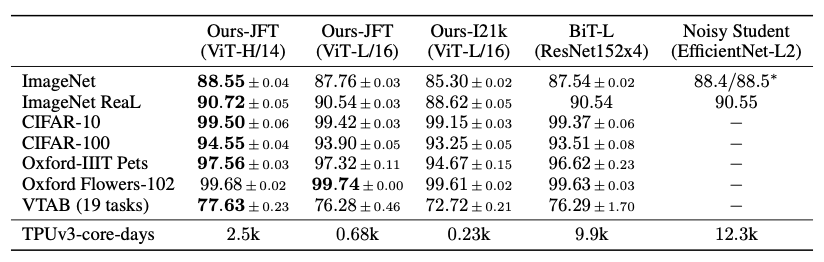
\includegraphics[width=1\textwidth]{img/3-section/Simple benchmark.png} 
\end{center}

Vision Transformer models pre-trained on the JFT-300M dataset outperform ResNet-based baselines on all datasets, while taking substantially less computational resources to pre-train

\end{frame}

\begin{frame}
\frametitle{Trained with different dataset}
Accuracy (\%) of Vision Transformer on various datasets when pretrained on ImageNet, ImageNet-21k or JFT300M
\begin{center}
    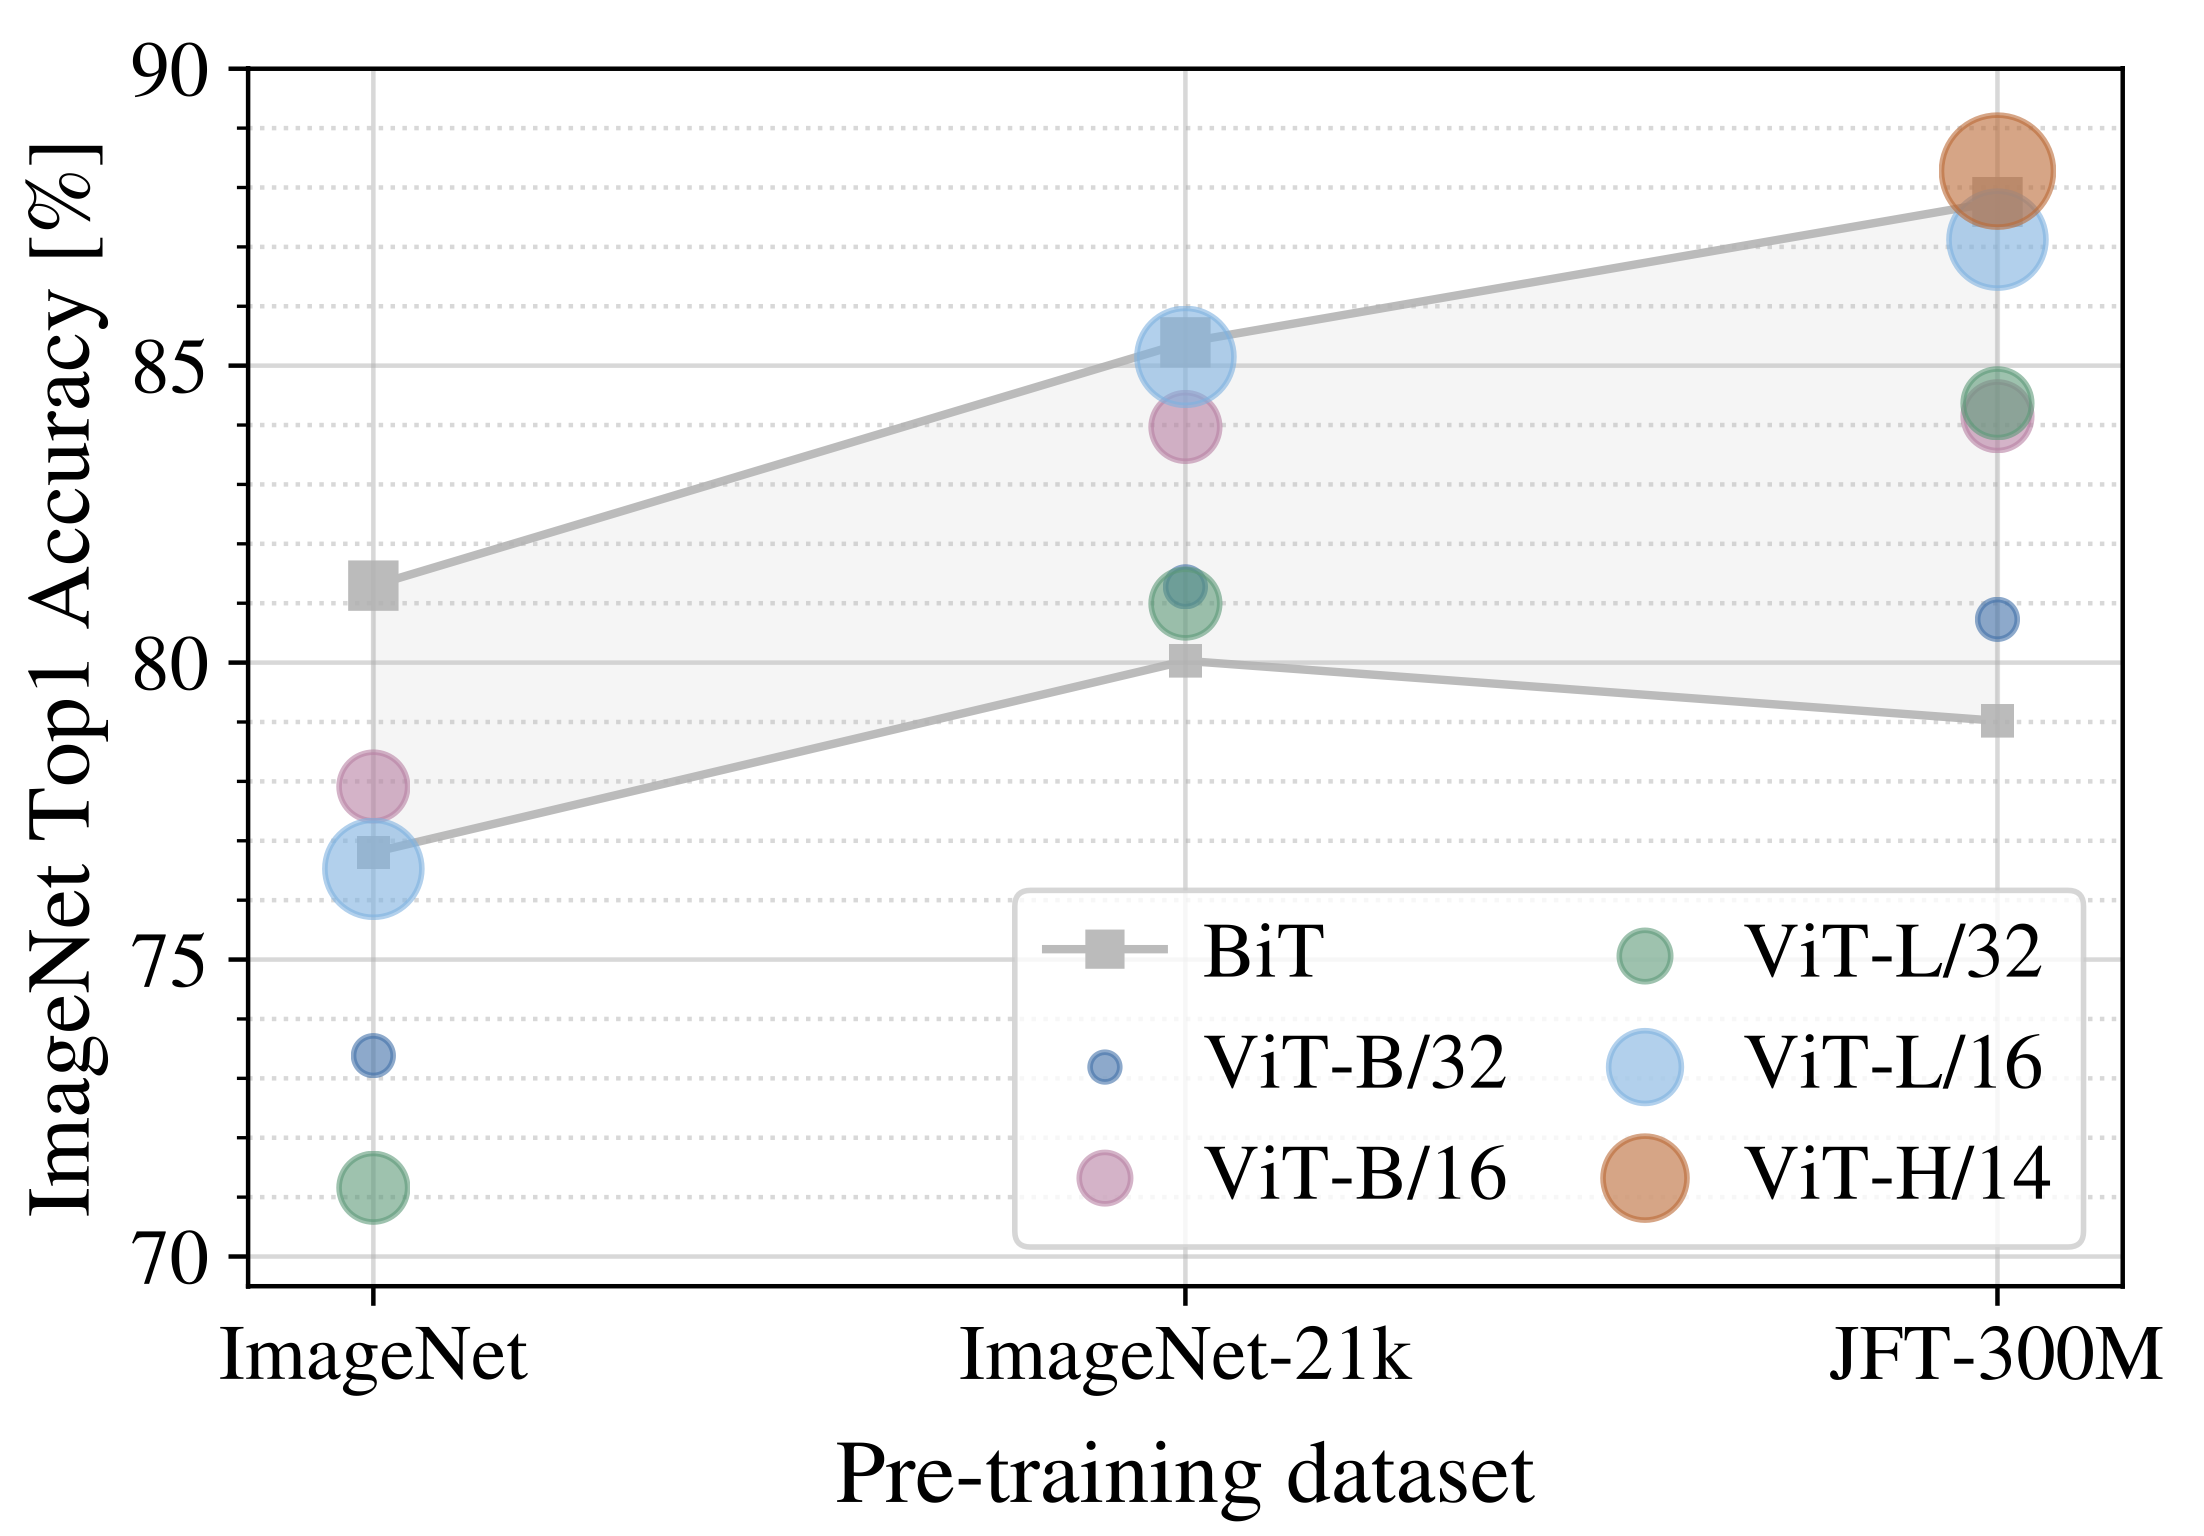
\includegraphics[width=0.5\textwidth]{img/3-section/Pretraining image.png} 
\end{center}
While large ViT models perform worse than BiT ResNets (shaded area) when pre-trained on small datasets, they \textbf{shine when pre-trained on larger datasets}. Similarly, larger ViT variants overtake smaller ones as the dataset grows.

\end{frame}


\begin{frame}
\frametitle{ConvNeXt by Facebook and Berkeley}
Reexamine the design space and push the limits of ConvNet potential, modernizing  standard ResNet towards a Transformer-like design, leading to the creation of ConvNeXt.

\begin{center}
    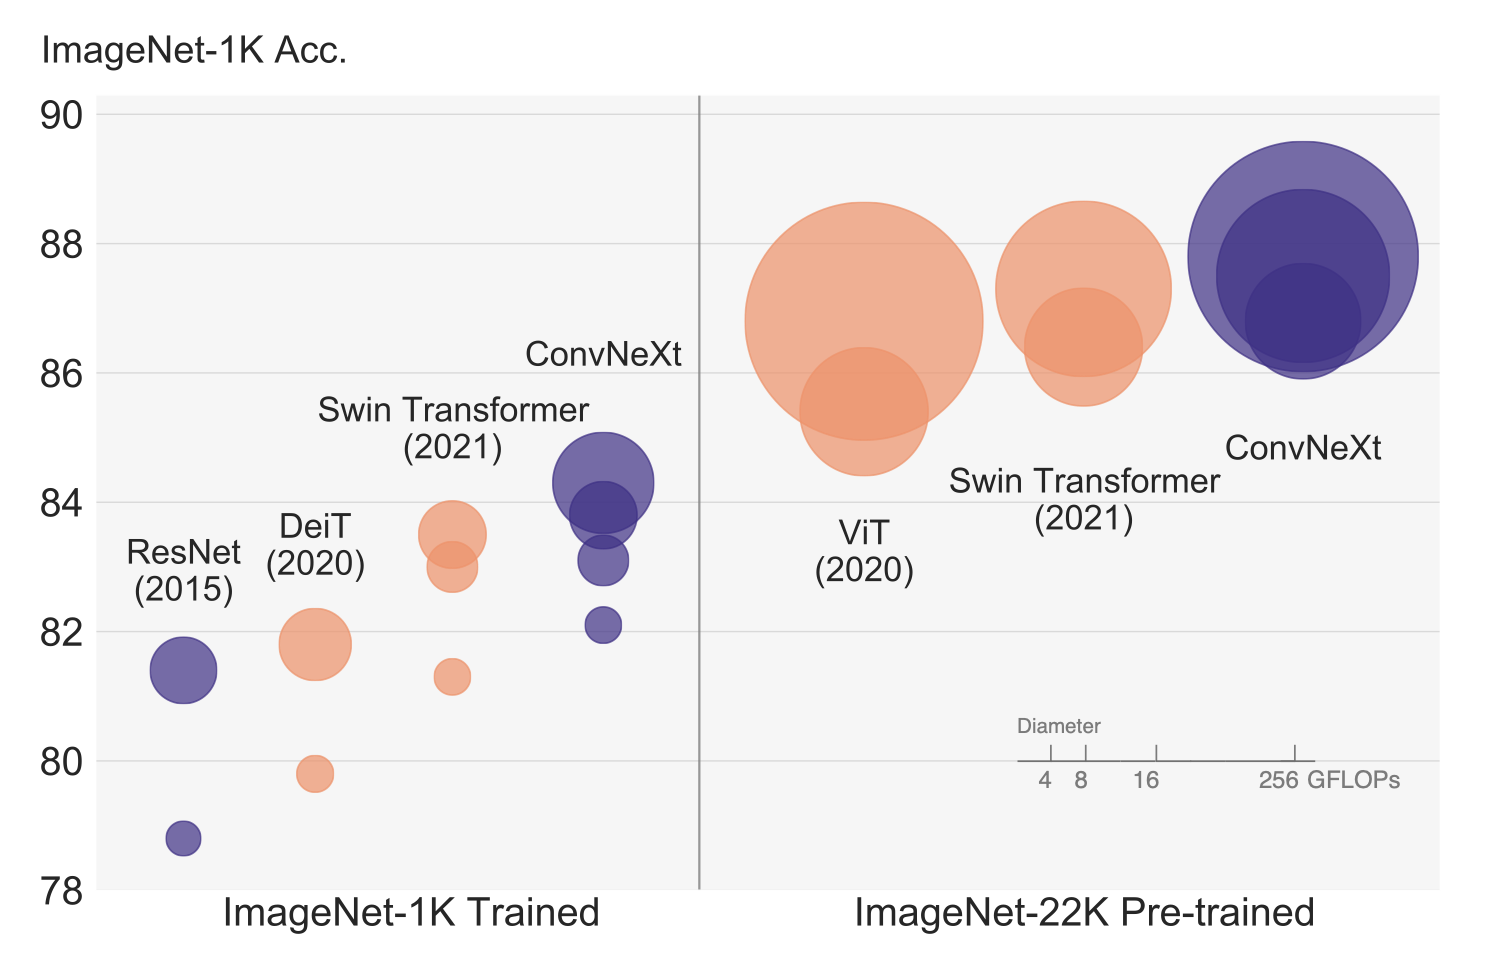
\includegraphics[width=0.7\textwidth]{img/3-section/ConvNext.png} 
\end{center}

\end{frame}

\begin{frame}
\frametitle{ConvNets Match Vision Transformers at Scale}
Google deepmind found out that ConvNets can match ViT at Scale

\vspace{0.5 cm}

\begin{center}
    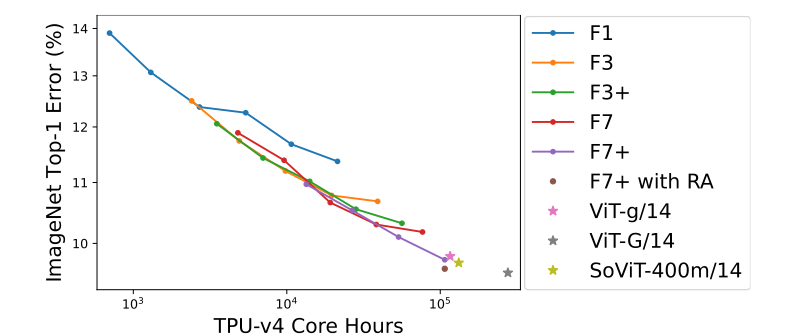
\includegraphics[width=0.7\textwidth]{img/3-section/log-log.png} 
\end{center}

Observed a log-log scaling law between held out loss (validation dataset) and compute budget.
\end{frame}

\begin{frame}
\frametitle{Key Observation, Google's point of view}

\vspace{0.5cm}
\begin{itemize}
    \item \textbf{Training Time:} The amount of computational resources and time dedicated to training the model
    \item \textbf{Dataset Quality and Size:} Access to large and diverse datasets, such as JFT-4B
\end{itemize}

\end{frame}


